\section{Expérimentation des chaînages avant}\label{sec:experimentation}
% les differentes experimentations faites pour comparer les differents chases
% commentaires pour chacun

Dans cette section nous présentons une évaluation exhaustive des différents \textit{chases}. Nous avons trois objectifs principaux en réalisant cette évaluation :

\begin{enumerate}
  \item Vérifier la correction des nos \textit{chases}.
  \item Comparer nos \textit{chases} à ceux qui existaient déjà dans Graal.
  \item Comparer tous les différents \textit{chases} implémentés. 
\end{enumerate}

\subsection{Méthode d'expérimentation}

Nous avons implémenté un outil de benchmarking qui nous permet de lancer tous les \textit{chases} (ceux que nous avons implémenté ainsi que ceux déjà existants dans Graal) avec des limites sur les temps globaux d'exécution, le temps d'exécution de chaque étape de largeur et le nombre des faits générés. Étant donné que les \textit{chases} peuvent facilement exploser en termes de temps d'exécution et de faits générés on a implémenté des limitations pour éviter d'obtenir des temps d'exécution trop longs et des possibles erreurs de mémoire. 

Le benchmark prends en entrée un fichier "dlp" avec la base des connaissances et lance chacun des \textit{chases} jusqu'à ce que la saturation se termine ou jusqu'à ce que l'une des trois conditions d'arrêt mentionnés précédemment soit atteinte. Une fois ce processus fini on sauvegarde comme résultat le temps d'exécution de chaque étape et le nombre de faits appartenant à la base de faits à la fin de chaque étape. Cela nous permets de faire des comparaisons détaillés entre tous les \textit{chases} exécutés.

%procède à la saturer itérativement avec chacun des chases jusqu'à ce que la saturation soit fini ou l'une des trois conditions d'arrêt mentionnés précédemment soit atteint.

Le nombre de faits générés nous permets de vérifier la correction de nos \textit{chases} par rapport a ceux existants dans Graal, une fois les \textit{chases} ont été corrigés le temps d'exécution nous permets de comparer l'efficacité de nos \textit{chases} par rapport à ceux déjà existants. Et finalement avec ces deux mesures nous pouvons aussi comparer tous les \textit{chases} en terme de vitesse d'exécution et de capacité à éviter des redondances.

\subsection{Bases de connaissances d'expérimentation}

Nous avons pris plusieurs bases de connaissances faites à la main pour tester les \textit{chases}, ces bases ont la particularité d'avoir peu de règles et peu des faits au départ tout en générant de nombreuses redondances. Cela nous permet de tester les limites des algorithmes après peu d'itérations. Nous avions aussi prévu d'exécuter des tests avec des bases de connaissances crées par la communauté scientifique dans le but explicite de pousser les algorithmes de \textit{chase} vers leurs limites. Malheureusement nous avons pas eu le temps de réaliser ces tests pendant le déroulement de ce TER, bien que certains de nos résultats soient intéressants, notre méthode de benchmark est assez naïve. Une batterie de tests plus soutenue sera donc à mettre en oeuvre pour améliorer la précision et la pertinence de nos résultats. Nos bases des connaissances d'expérimentation sont les suivants : 

\vspace{10pt}
\textbf{$\mathcal{KB}_A$}\\
$\mathcal{F} = \{p(a,b)\}$ \\
$R = p(X,Y) \rightarrow p(Y,Z), p(Z,Z), p(Z,X), p(X,U), p(U,Y), p(U,U)$\\

\textbf{$\mathcal{KB}_B$}\\
$\mathcal{F} = \{p(a,b)\}$ \\
$R = p(X,Y) \rightarrow p(Y,Z), p(Z,U), p(U,X), p(X,O), p(O,Q), p(Q,Y), p(U,U), p(Q,Q), p(O,O), p(Z,Z)$\\

\textbf{$\mathcal{KB}_C$}\\
$\mathcal{F} = \{p(c,d), p(a,b), p(e,f)\}$ \\
$R = p(X,Y), p(U,W) \rightarrow q(X,Z), q(Z,X), p(Z,V), q(U,Z), q(Z,U)$\\

\textbf{$\mathcal{KB}_D$}\\
$\mathcal{F} = \{p1(a), p1(n),q(b,f),q(f,c),q(b7,f5),q(f5,c5),q(b6,f6),q(f8,c8)\}$ \\
$R = p1(X), q(V,Y) \rightarrow p1(Z),p(X,Z),q(V,Z)$\\

\textbf{$\mathcal{KB}_E$}\\
$\mathcal{F} = \{b(a), c(a)\}$\\
$R1 = b(X) \rightarrow p(X,Z)$\\
$R2 = p(X,Y) \rightarrow p(X,Z), a(Z)$\\
$R3 = p(X,Y), a(W) \rightarrow p(Y,Z)$\\
$R4 = p(X,Y), a(Y) \rightarrow p(Y,Y)$\\
$R5 = p(X,Y), c(X) \rightarrow q(Y)$\\

\textbf{$\mathcal{KB}_F$}\\
$\mathcal{F} = \{p(a,b), p(b,c), p(c,d)\}$\\
$R = p(X,Y) \rightarrow p(Y,Z), p(Z,Z), p(Z,X), p(X,U), p(U,Y), p(U,V), p(V,Z), p(V,V), p(X,A), p(A,B), p(B,Y)$

\subsection{Résultats}

Toutes les expérimentations ont été réalisés sur un seul ordinateur avec un processeur AMD FX-8350 et 16Go de mémoire. Les paramètres d'arrêt utilisés lors du benchmark sont 1 heure de temps de exécution globale, 30 minutes maximum par étape et 1.000.000 de faits générés.

\subsubsection{Comparaison Graal Chases et Nouveaux Chases}
Nous commençons pour vérifier la correction de nos algorithmes, pour ce faire nous avons lancé le benchmark pour les 6 bases de connaissances mentionnés précédemment et nous comparons le nombre de faits générés à la dernière étape par tous les algorithmes. Les résultats sont présentés dans le tableau \ref{tab:faitsoldnew}.


\begin{table}[H]
\begin{center}
\begin{tabular}{|c|c|c|c|c|} 
    \hline
    $\mathcal{KB}$/Étape & \shortstack{New \\ Semi-oblivious Chase}  & \shortstack{Graal \\ Semi-oblivious Chase} & \shortstack{New \\ Parallel Restricted Chase} & \shortstack{Graal \\ Parallel Restricted Chase} \\
    \hline
     \hline
    $\mathcal{KB}_A$/6 & 55987 & 55987 & 1375 & 1375 \\ 
     \hline
    $\mathcal{KB}_B$/5 & 111111 & 111111 & 3851 & 3851 \\ 
    \hline
    $\mathcal{KB}_C$/4 & 107754 & 107754 & 21882 & 21882 \\ 
    \hline
    $\mathcal{KB}_D$/4 & 1556 & 1556 & 1556 & 152324 \\ 
    \hline
    $\mathcal{KB}_E$/13 & 754 & 754 & 332 & 332 \\ 
     \hline
    $\mathcal{KB}_F$/4 & 48315 & 48315 & 24918 & 24918 \\ 
     \hline 
\end{tabular}    
\caption {Comparaison \textit{Graal Chases} - \textit{Nouveaux Chases}} \label{tab:faitsoldnew}
\end{center}
\end{table}

Les résultats sont correct, en effet, nous pouvons constater que le \textit{graal semi-oblivious chase} et le \textit{nouveau semi-oblivious chase} génèrent la même quantité d'atomes, le \textit{graal restricted chase} et le \textit{nouveau restricted chase} génerènt aussi la même quantité d'atomes sauf dans le cas du $\mathcal{KB}_D$ où le \textit{graal restricted chase} génère même plus d'atomes que le \textit{graal semi-oblivious chase}. Cela s'explique car il y a un bug dans la classe BacktrackHomomorphism de Graal.

Maintenant que nous avons validé la correction de nos \textit{chases}, nous allons comparer les temps d'exécution du \textit{semi-oblivious chase} et \textit{restricted chase} qui sont implémentés dans Graal avec nos nouvelles versions. Les graphiques présentées ci-dessous montrent le temps en millisecondes (axe Y) en fonction de l'étape de largeur (axe X). L'axe temps a été mis en échelle avec une fonction logarithme pour que les graphes restent lisibles. Les tableaux utilisés pour construire tous ces graphiques se trouvent dans l'annexe B.

Prenons les résultats de $\mathcal{KB}_A$ (Fig. \ref{fig:ex0oldnew}), nous pouvons voir que dans le cas du \textit{semi-oblivious chase} la nouvelle implémentation est plus lente que celle de Graal lors des premières étapes quand la base des faits est petite, après quand la base de faits commence à grandir la nouvelle implementation deviens considérablement plus rapide. On remarque que l'implementation de Graal fait un timeout pendant le calcul de l'étape 7, ce qui explique que la courbe fini à l'étape 6, alors que la nouvelle implémentation arrive à calculer deux étapes de plus. Nous observons des résultats similaires avec le \textit{restricted chase}, c'est un peu difficile à constater dans le graphique due à l'échelle logarithmique utilisé mais le \textit{nouvel restricted chase} a réalisé 12 étapes de largeur en 23 minutes tandis que la version de Graal a mis 25 minutes et demi pour faire le même calcul. Cette amélioration en temps de calcul est due principalement à notre méthode de calcul des nouveaux homomorphismes qui nous évite de faire des calculs redondants tandis-que que l'implémentation de Graal calcule tous les homomorphismes à chaque étape de largeur.

\begin{figure}
\centering
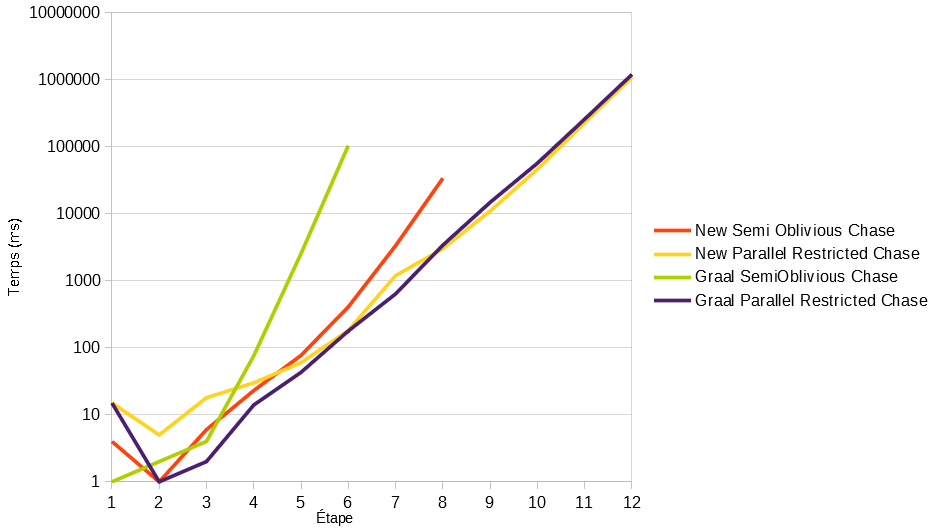
\includegraphics[width=\textwidth]{pictures/benchmark_old-new/ex0oldnew.png}
\caption{$\mathcal{KB}_A$ }
\label{fig:ex0oldnew}
\end{figure}

\begin{figure}
\centering
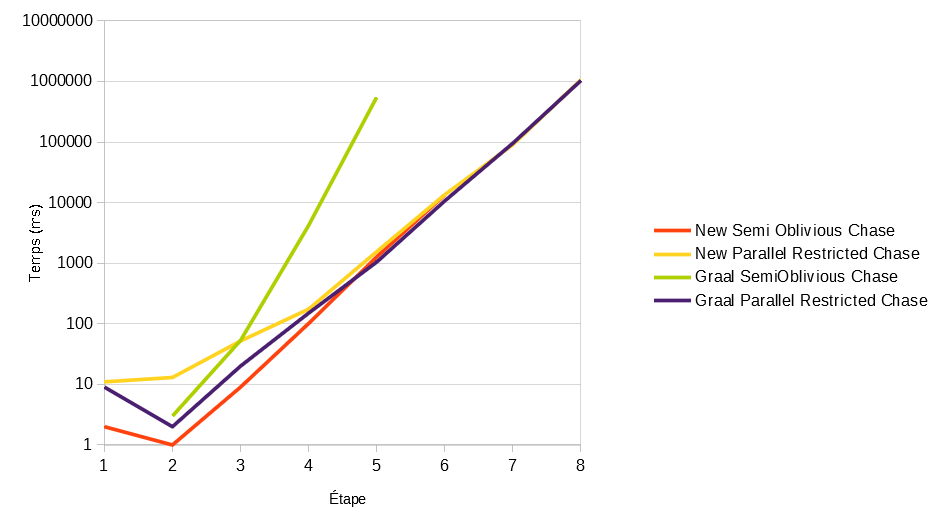
\includegraphics[width=\textwidth]{pictures/benchmark_old-new/ex1oldnew.png}
\caption{$\mathcal{KB}_B$}
\label{fig:ex1oldnew}
\end{figure}

\begin{figure}
\centering
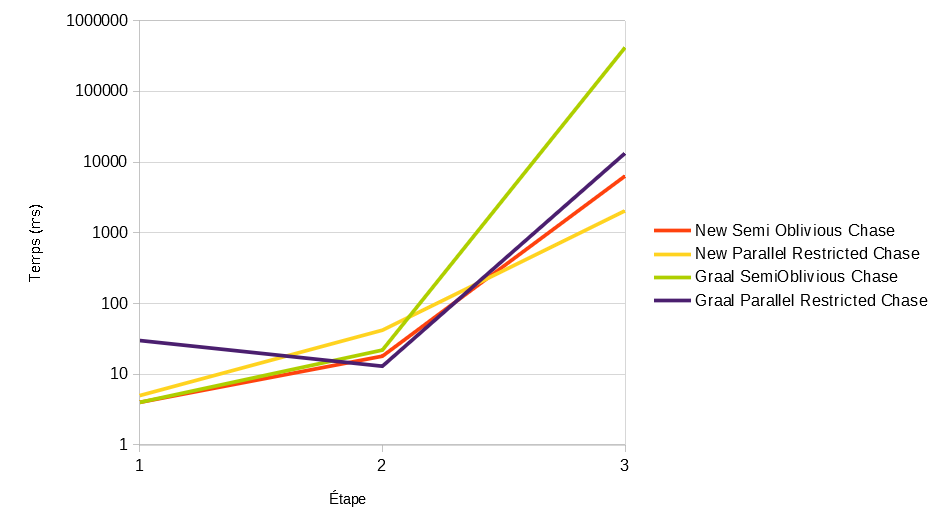
\includegraphics[width=\textwidth]{pictures/benchmark_old-new/ex2oldnew.png}
\caption{$\mathcal{KB}_C$}
\label{fig:ex2oldnew}
\end{figure}

\begin{figure}
\centering
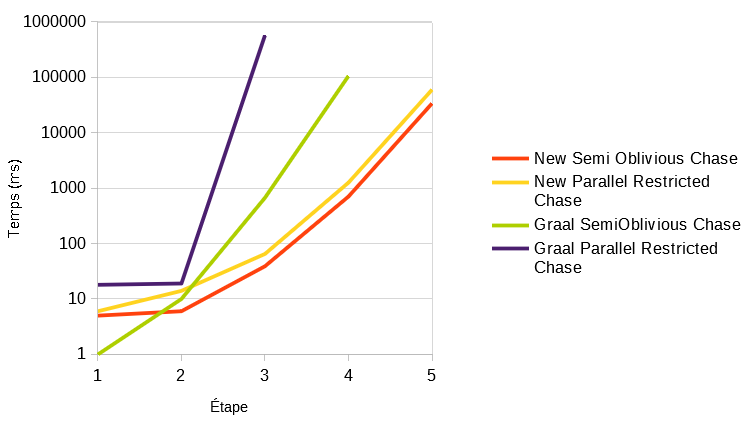
\includegraphics[width=\textwidth]{pictures/benchmark_old-new/ex11oldnew.png}
\caption{$\mathcal{KB}_D$}
\label{fig:ex11oldnew}
\end{figure}

\begin{figure}
\centering
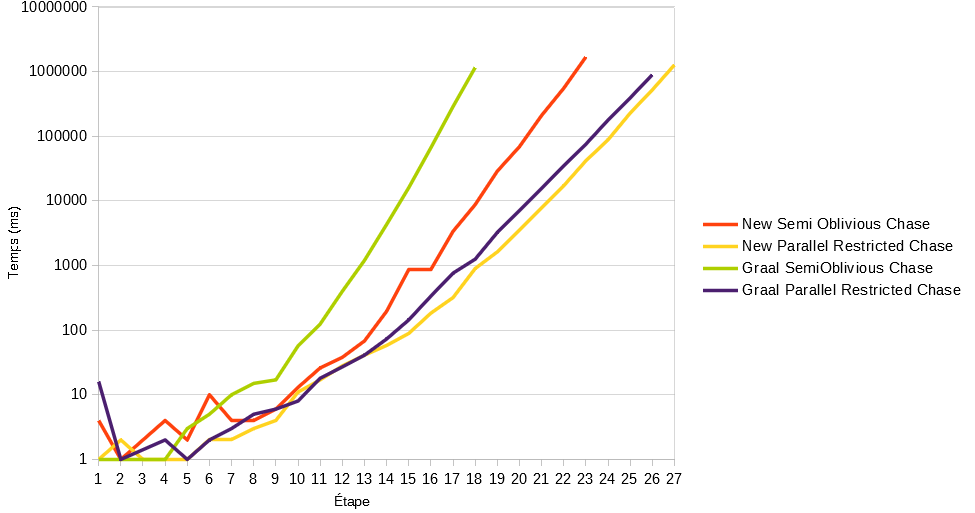
\includegraphics[width=\textwidth]{pictures/benchmark_old-new/exampleoldnew.png}
\caption{$\mathcal{KB}_E$}
\label{fig:exampleoldnew}
\end{figure}

\begin{figure}
\centering
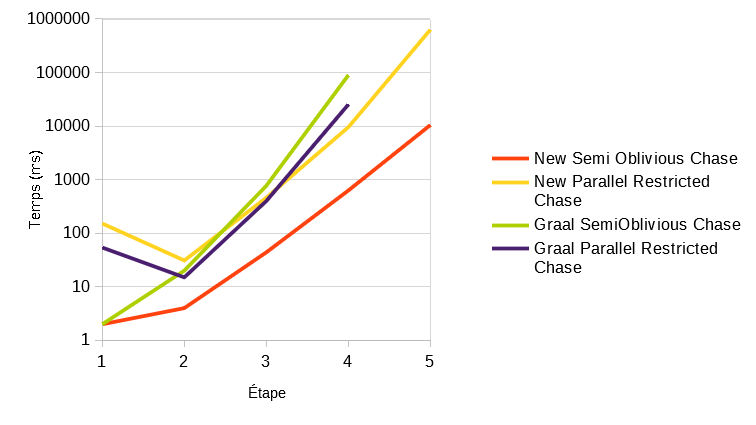
\includegraphics[width=\textwidth]{pictures/benchmark_old-new/moldnew.png}
\caption{$\mathcal{KB}_F$}
\label{fig:moldnew}
\end{figure}

Nous observons des résultats similaires dans les autres exemples, avec deux exceptions à noter, premièrement, dans $\mathcal{KB}_B$ (Fig. \ref{fig:ex1oldnew}) le \textit{nouvel restricted chase} prends 27 secondes de plus pour calculer 12 étapes que le \textit{restricted chase} de Graal, cela peut s'expliquer dpar le fait que l'on a pris qu'une seule mesure, en refaisant l'expérimentation ou en la laissant tourner une étape de plus on devrait atteindre de meilleurs résultats. Deuxièmement, dans $\mathcal{KB}_D$ le temps de calcul du \textit{restricted chase} de Graal augmente de façon exponentielle due au bug trouvé dans la classe BacktrackHomomorphism de Graal.

Après avoir réalisés ces expérimentations nous pouvons conclure que notre implémentation des \textit{chases} montrent des résultats satisfaisants qui se démarque au fur et au mesure que la base de faits qu'on est en train de saturer grandis. 

\subsubsection{Comparaison Nouveaux Chases}

Maintenant nous allons comparer tous les chases que nous avons implementé, c'est-à-dire, les nouvelles versions du \textit{restricted chase}, le \textit{core chase}, le \textit{local core chase} et le \textit{vacuum chase}. La méthode employé ici est la même que précédemment mais nous cherchons plutôt ici à comparer les différents types de \textit{chase}.

Avec la base de connaissances $\mathcal{KB}_A$ (Fig. \ref{fig:ex0newfacts} et  Fig. \ref{fig:ex0newtime}) nous observons que le \textit{local core chase} et le \textit{core chase} finissent la saturation lors de l'étape 4 avec 31 faits générés, la différence de temps entre les deux n'est pas significative dans cette exemple. Le \textit{vacuum chase} et le \textit{parallel restricted chase} montrent des résultats similaires jusqu'à l'étape 6, lors de l'étape 7 le \textit{vacuum chase} semble même être meilleur pendant un temps avant de se mettre à générer plus des redondances que le \textit{restricted chase}. Cette irrégularité semble indiqué un problème avec notre implémentation du \textit{vacuum chase}. 

\begin{figure}
\centering
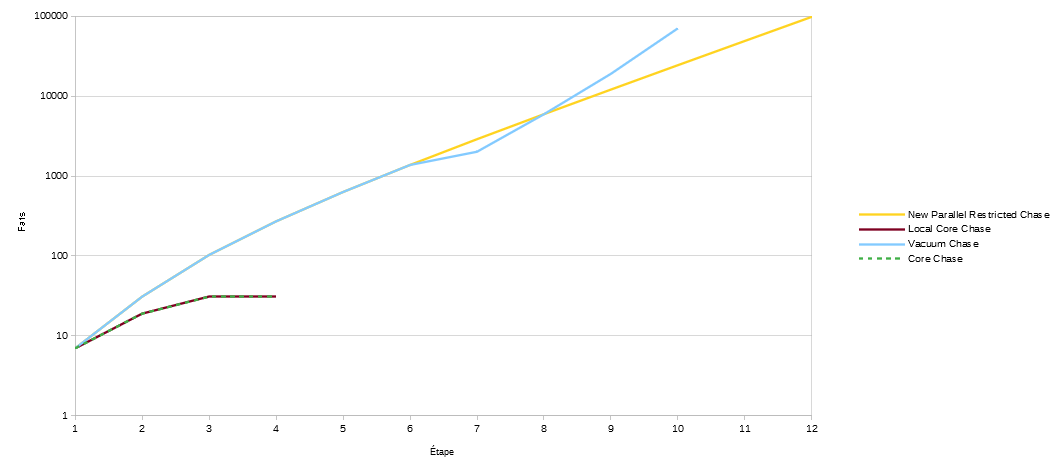
\includegraphics[width=\textwidth]{pictures/benchmark_new/ex0newfacts.png}
\caption{$\mathcal{KB}_A$ Faits générés}
\label{fig:ex0newfacts}
\end{figure}

\begin{figure}
\centering
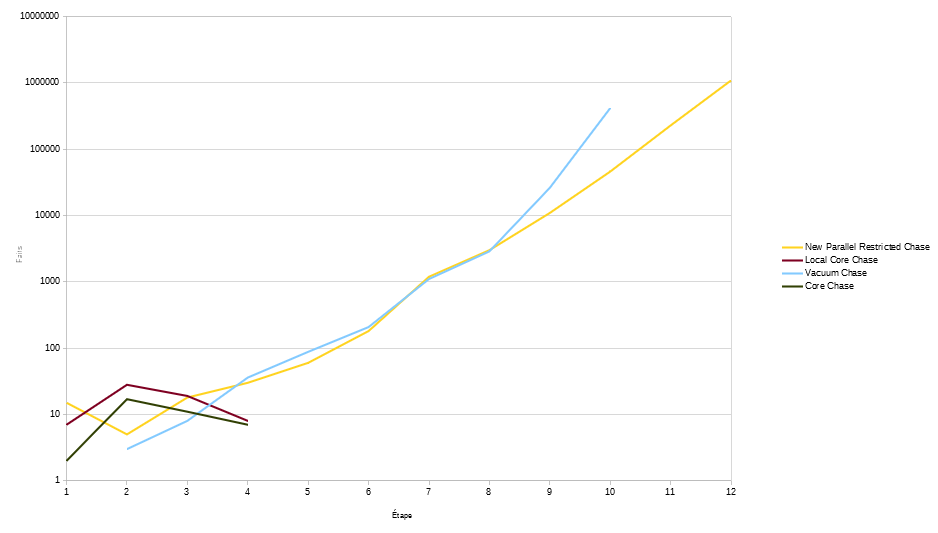
\includegraphics[width=\textwidth]{pictures/benchmark_new/ex0newtime.png}
\caption{$\mathcal{KB}_A$ Temps}
\label{fig:ex0newtime}
\end{figure}

Dans la base de connaissances $\mathcal{KB}_E$ (Fig. \ref{fig:examplenewfacts} et  Fig. \ref{fig:examplenewtime}) nous pouvons remarquer que l'algorithme qui prend le plus de temps c'est le \textit{parallel restricted chase}, cela est du au fait qu'il génère de nombreux faits redondants. Le \textit{vacuum chase}, lui, est capable d'éliminer un grand nombre des faits redondants ce qui le rends plus efficace que le \textit{parallel restricted chase} en temps d'exécution aussi qu'en quantité des faits générés. Le \textit{local core chase} et le \textit{breadth first restricted chase}, eux, sont équivalents en termes de faits produits, cela peut s'expliquer par le fait que le \textit{breadth first restricted chase} a un ordre d'application des règles qui est équivalent au \textit{local core chase}. Comme attendu le \textit{breadth first chase} est beacoup plus rapide que le \textit{local core chase} car il fait moins des calculs. Finalement, Le \textit{core chase}, fini ici en 5 étapes avec une base de faits contenant 6 faits ce qui fait de lui l'algorithme le plus efficace en nombre de faits produits. Il obtient aussi le meilleur temps car, contrairement aux autres algorithmes, il fini sa saturation.

\begin{figure}
\centering
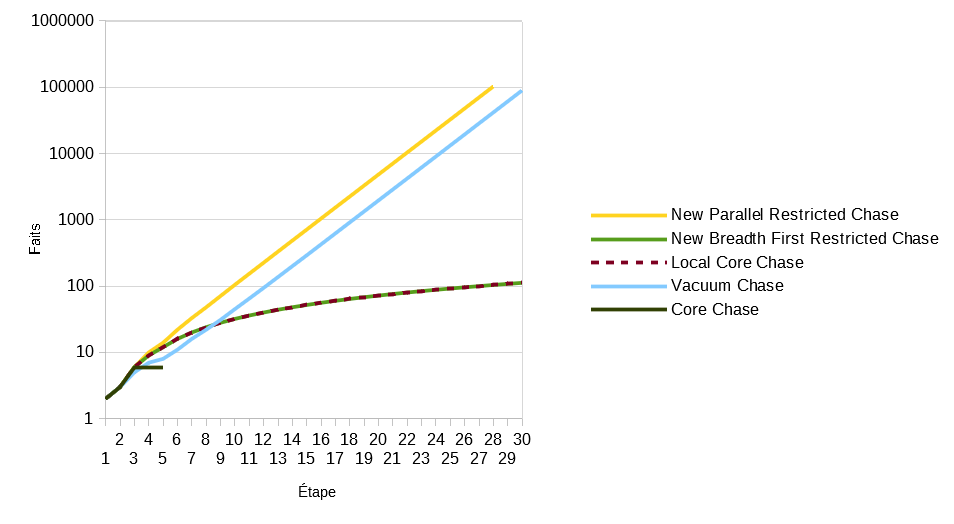
\includegraphics[width=\textwidth]{pictures/benchmark_new/examplenewfacts.png}
\caption{$\mathcal{KB}_E$ Faits générés}
\label{fig:examplenewfacts}
\end{figure}

\begin{figure}
\centering
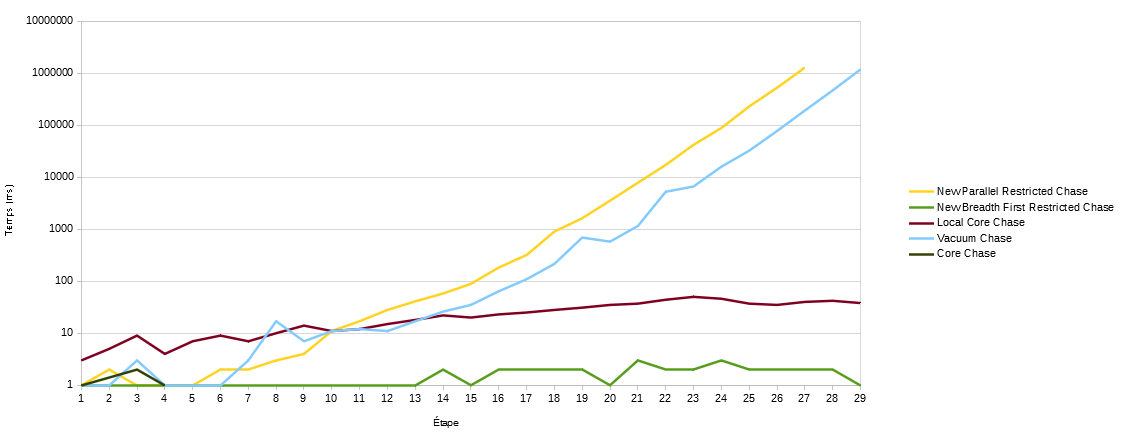
\includegraphics[width=\textwidth]{pictures/benchmark_new/examplenewtimes.png}
\caption{$\mathcal{KB}_E$ Temps}
\label{fig:examplenewtime}
\end{figure}

Puis, en utilisant $\mathcal{KB}_F$ (Fig. \ref{fig:mnewtime} et Fig. \ref{fig:mnewfacts}) nous observons que le \textit{core chase} arrive à enlever plus des redondances que le \textit{local core chase}, néanmoins ce dernier reste beaucoup plus rapide. Il prends 6 minutes et demi pour finir 3 étapes de largeur pendant que le \textit{core chase} à besoin d'environ 16 minutes. Il faut remarquer que les deux algorithmes font un timeout l'étape 4 leurs prenant plus de 30 minutes. Le \textit{vacuum chase} arrive à enlever des redondances que le \textit{parallel restricted chase} n'est pas capable de détecter, néanmoins il est considérablement plus lent. en fait il n'arrive à finir que 4 étapes de largeur avant d'atteindre le timeout tandis que le \textit{parallel restricted chase} a pu finir 5 étapes de largeur. 
%à besoin d'environ 16 minutes pour calculer 6 étapes ( faux il me semble que c'est 3 étapes a vérifier!)

\begin{figure}
\centering
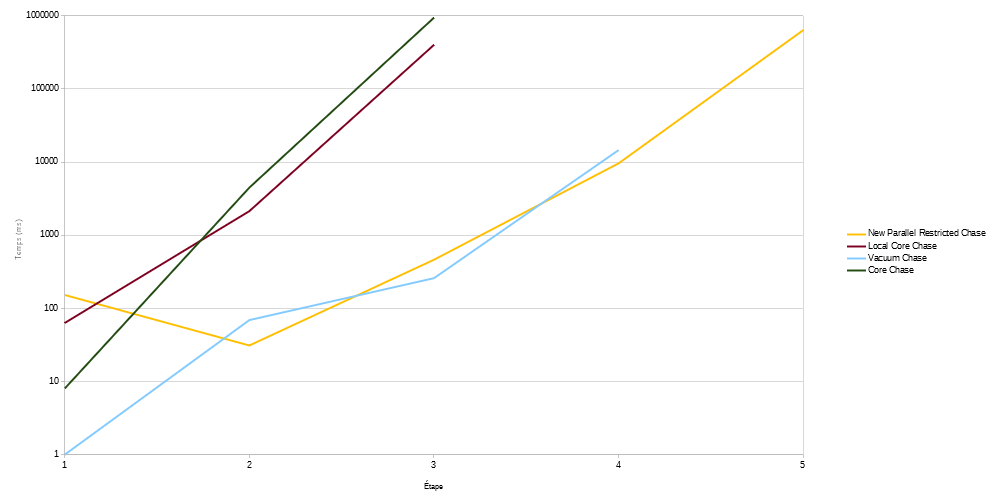
\includegraphics[width=\textwidth]{pictures/benchmark_new/mnewtimes.png}
\caption{$\mathcal{KB}_F$ Temps}
\label{fig:mnewtime}
\end{figure}

\begin{figure}
\centering
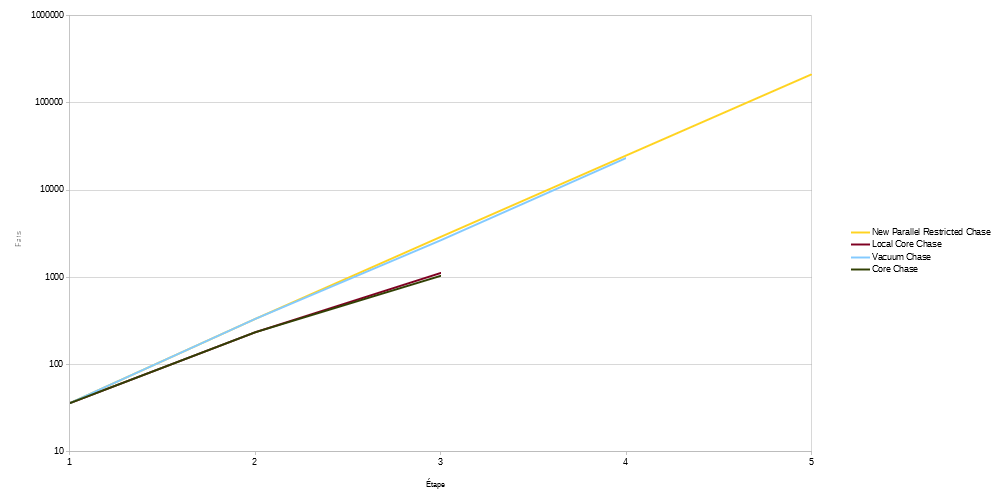
\includegraphics[width=\textwidth]{pictures/benchmark_new/mnewfacts.png}
\caption{$\mathcal{KB}_F$ Faits générés}
\label{fig:mnewfacts}
\end{figure}

Nous pouvons observer que le \textit{local core chase} et le \textit{vacuum chase} se trouvent entre le \textit{restricted chase} et le \textit{core chase}, en termes de temps mais aussi en termes de redondances détectés. il faut aussi remarquer que de façon général le \textit{local core chase} élimine plus de redondances que le \textit{vacuum chase} mais il est aussi plus lent. Le calcul du core reste un calcul compliqué même quand la base de faits est pré-gelée. Dans les cas où le calcul du core permets l'arrêt de la saturation, le \textit{core chase} est l'algorithme le plus puissant.

\par Après avoir étudié la suppression des redondances dans le cadre du chaînage avant, on va présenter la suppression des redondances dans les règles.